% Data-derived TikZ; the main document supplies the same font as Figure 2.
\definecolor{hcinitial}{HTML}{A37545}
\definecolor{hcind}{HTML}{78818E}
\definecolor{hcevo}{HTML}{00858B}
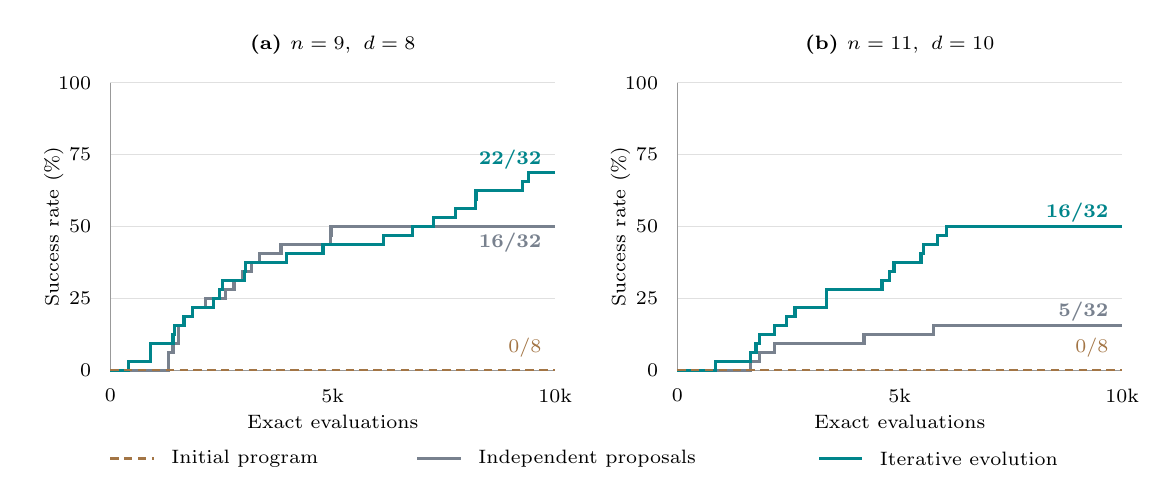
\begin{tikzpicture}[x=1cm,y=1cm,font=\scriptsize,baseline]
\path[use as bounding box] (-1.05,-1.32) rectangle (13.15,4.35);
\begin{scope}[xshift=0cm]
\node[font=\scriptsize\bfseries] at (2.825,4.14) {(a) $n=9,\ d=8$};
\draw[black!12,line width=.35pt] (0,0.0)--(5.65,0.0);
\node[anchor=east] at (-.12,0.0) {0};
\draw[black!12,line width=.35pt] (0,0.9125)--(5.65,0.9125);
\node[anchor=east] at (-.12,0.9125) {25};
\draw[black!12,line width=.35pt] (0,1.825)--(5.65,1.825);
\node[anchor=east] at (-.12,1.825) {50};
\draw[black!12,line width=.35pt] (0,2.7375)--(5.65,2.7375);
\node[anchor=east] at (-.12,2.7375) {75};
\draw[black!12,line width=.35pt] (0,3.65)--(5.65,3.65);
\node[anchor=east] at (-.12,3.65) {100};
\draw[black!40,line width=.4pt] (0,3.65)--(0,0)--(5.65,0);
\node[rotate=90] at (-.72,1.825) {Success rate (\%)};
\node at (2.825,-.66) {Exact evaluations};
\node[anchor=north] at (0,-.12) {0};
\node[anchor=north] at (2.825,-.12) {5k};
\node[anchor=north] at (5.65,-.12) {10k};
\draw[hcind,line width=1.15pt] (0.00000,0.00000) -- (0.74241,0.00000) -- (0.74241,0.22812) -- (0.79495,0.22812) -- (0.79495,0.34219) -- (0.86332,0.34219) -- (0.86332,0.57031) -- (0.93621,0.57031) -- (0.93621,0.68437) -- (1.04582,0.68437) -- (1.04582,0.79844) -- (1.21249,0.79844) -- (1.21249,0.91250) -- (1.46166,0.91250) -- (1.46166,1.02656) -- (1.57014,1.02656) -- (1.57014,1.14062) -- (1.67975,1.14062) -- (1.67975,1.25469) -- (1.79614,1.25469) -- (1.79614,1.36875) -- (1.88993,1.36875) -- (1.88993,1.48281) -- (2.16621,1.48281) -- (2.16621,1.59688) -- (2.80071,1.59688) -- (2.80071,1.71094) -- (2.80296,1.71094) -- (2.80296,1.82500) -- (5.65000,1.82500);
\node[anchor=east,text=hcind,font=\scriptsize\bfseries] at (5.60,1.61500) {16/32};
\draw[hcevo,line width=1.15pt] (0.00000,0.00000) -- (0.23561,0.00000) -- (0.23561,0.11406) -- (0.50737,0.11406) -- (0.50737,0.22812) -- (0.51076,0.22812) -- (0.51076,0.34219) -- (0.79495,0.34219) -- (0.79495,0.45625) -- (0.81417,0.45625) -- (0.81417,0.57031) -- (0.93621,0.57031) -- (0.93621,0.68437) -- (1.04582,0.68437) -- (1.04582,0.79844) -- (1.31024,0.79844) -- (1.31024,0.91250) -- (1.38877,0.91250) -- (1.38877,1.02656) -- (1.42719,1.02656) -- (1.42719,1.14062) -- (1.69952,1.14062) -- (1.69952,1.25469) -- (1.71873,1.25469) -- (1.71873,1.36875) -- (2.23627,1.36875) -- (2.23627,1.48281) -- (2.70070,1.48281) -- (2.70070,1.59688) -- (3.47249,1.59688) -- (3.47249,1.71094) -- (3.83805,1.71094) -- (3.83805,1.82500) -- (4.10868,1.82500) -- (4.10868,1.93906) -- (4.37875,1.93906) -- (4.37875,2.05313) -- (4.63413,2.05313) -- (4.63413,2.16719) -- (4.64430,2.16719) -- (4.64430,2.28125) -- (5.23021,2.28125) -- (5.23021,2.39531) -- (5.31439,2.39531) -- (5.31439,2.50937) -- (5.65000,2.50937);
\node[anchor=east,text=hcevo,font=\scriptsize\bfseries] at (5.60,2.67937) {22/32};
\draw[hcinitial,line width=.9pt,dash pattern=on 3pt off 2pt] (0.00000,0.00000) -- (5.65000,0.00000);
\node[anchor=south east,text=hcinitial] at (5.60,0.04000) {0/8};
\end{scope}
\begin{scope}[xshift=7.2cm]
\node[font=\scriptsize\bfseries] at (2.825,4.14) {(b) $n=11,\ d=10$};
\draw[black!12,line width=.35pt] (0,0.0)--(5.65,0.0);
\node[anchor=east] at (-.12,0.0) {0};
\draw[black!12,line width=.35pt] (0,0.9125)--(5.65,0.9125);
\node[anchor=east] at (-.12,0.9125) {25};
\draw[black!12,line width=.35pt] (0,1.825)--(5.65,1.825);
\node[anchor=east] at (-.12,1.825) {50};
\draw[black!12,line width=.35pt] (0,2.7375)--(5.65,2.7375);
\node[anchor=east] at (-.12,2.7375) {75};
\draw[black!12,line width=.35pt] (0,3.65)--(5.65,3.65);
\node[anchor=east] at (-.12,3.65) {100};
\draw[black!40,line width=.4pt] (0,3.65)--(0,0)--(5.65,0);
\node[rotate=90] at (-.72,1.825) {Success rate (\%)};
\node at (2.825,-.66) {Exact evaluations};
\node[anchor=north] at (0,-.12) {0};
\node[anchor=north] at (2.825,-.12) {5k};
\node[anchor=north] at (5.65,-.12) {10k};
\draw[hcind,line width=1.15pt] (0.00000,0.00000) -- (0.93056,0.00000) -- (0.93056,0.11406) -- (1.04356,0.11406) -- (1.04356,0.22812) -- (1.23679,0.22812) -- (1.23679,0.34219) -- (2.37074,0.34219) -- (2.37074,0.45625) -- (3.25327,0.45625) -- (3.25327,0.57031) -- (5.65000,0.57031);
\node[anchor=east,text=hcind,font=\scriptsize\bfseries] at (5.60,0.74031) {5/32};
\draw[hcevo,line width=1.15pt] (0.00000,0.00000) -- (0.48251,0.00000) -- (0.48251,0.11406) -- (0.93056,0.11406) -- (0.93056,0.22812) -- (0.99892,0.22812) -- (0.99892,0.34219) -- (1.04356,0.34219) -- (1.04356,0.45625) -- (1.23679,0.45625) -- (1.23679,0.57031) -- (1.38199,0.57031) -- (1.38199,0.68437) -- (1.49386,0.68437) -- (1.49386,0.79844) -- (1.89671,0.79844) -- (1.89671,0.91250) -- (1.89953,0.91250) -- (1.89953,1.02656) -- (2.59900,1.02656) -- (2.59900,1.14062) -- (2.69787,1.14062) -- (2.69787,1.25469) -- (2.75325,1.25469) -- (2.75325,1.36875) -- (3.09451,1.36875) -- (3.09451,1.48281) -- (3.12445,1.48281) -- (3.12445,1.59688) -- (3.30356,1.59688) -- (3.30356,1.71094) -- (3.41542,1.71094) -- (3.41542,1.82500) -- (5.65000,1.82500);
\node[anchor=east,text=hcevo,font=\scriptsize\bfseries] at (5.60,1.99500) {16/32};
\draw[hcinitial,line width=.9pt,dash pattern=on 3pt off 2pt] (0.00000,0.00000) -- (5.65000,0.00000);
\node[anchor=south east,text=hcinitial] at (5.60,0.04000) {0/8};
\end{scope}
\draw[hcinitial,line width=1pt,dash pattern=on 3pt off 2pt] (0,-1.12)--(0.55,-1.12);
\node[anchor=west] at (0.65,-1.12) {Initial program};
\draw[hcind,line width=1pt] (3.9,-1.12)--(4.45,-1.12);
\node[anchor=west] at (4.55,-1.12) {Independent proposals};
\draw[hcevo,line width=1pt] (9.0,-1.12)--(9.55,-1.12);
\node[anchor=west] at (9.65,-1.12) {Iterative evolution};
\end{tikzpicture}
